\documentclass{standalone}
\usepackage{tikz}
\usetikzlibrary{patterns, positioning}

\begin{document}
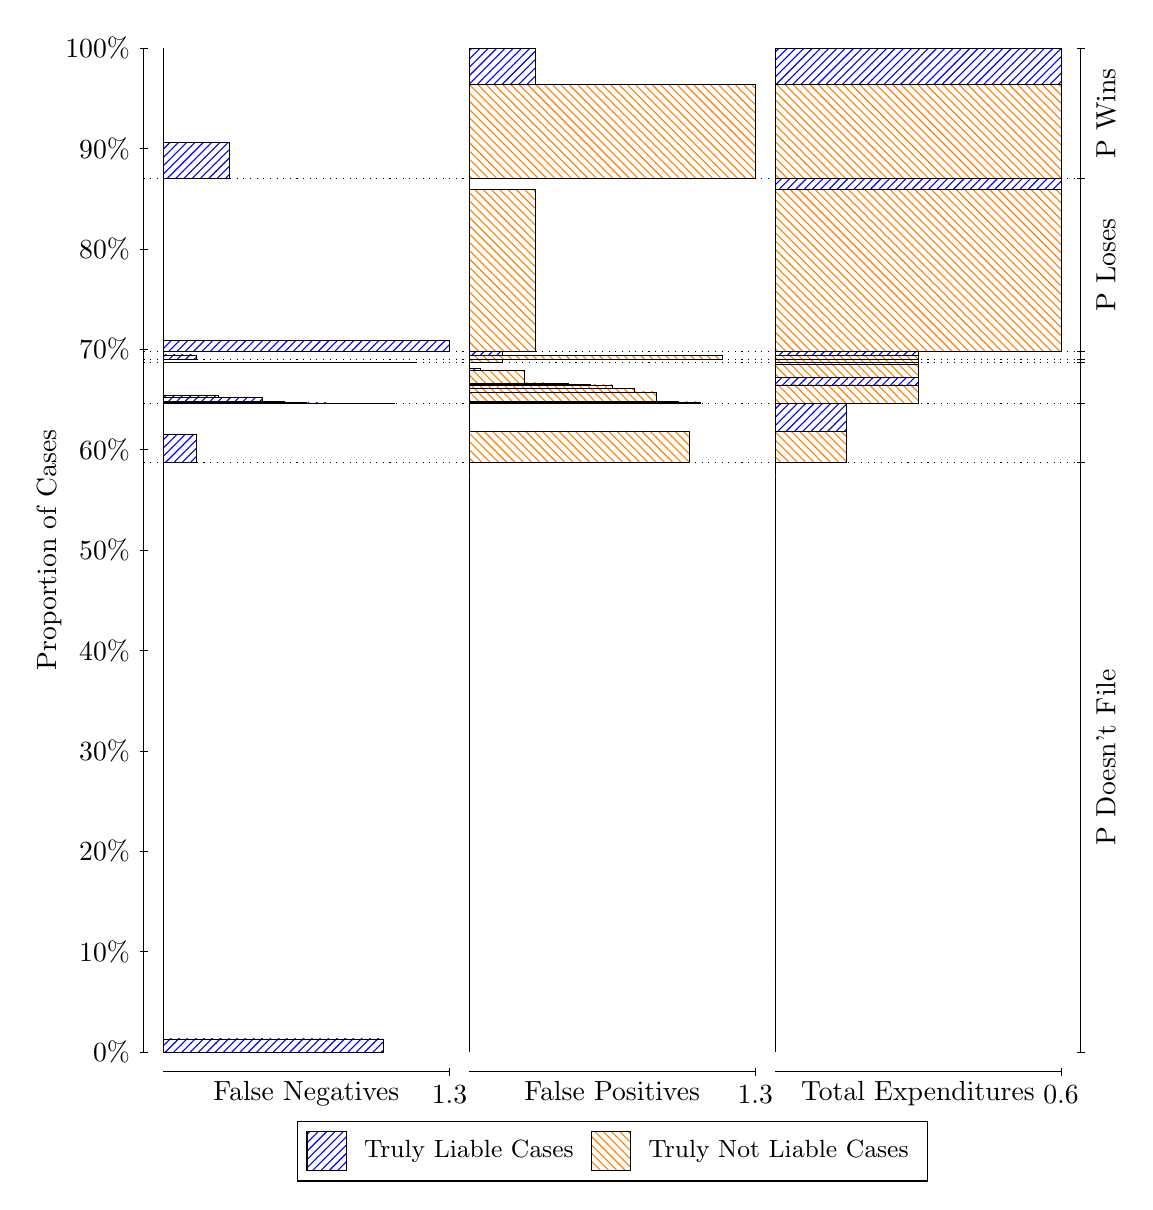
\begin{tikzpicture}
\draw[black, very thin] (1.5,1.75) -- (1.5,14.5);
\node[rotate=90, anchor=center] at (0.3, 8.125) {Proportion of Cases};
\draw[black, very thin] (1.45,1.75) -- (1.55,1.75);
\node[anchor=east] at (1.45, 1.75) {0\%};
\draw[black, very thin] (1.45,3.025) -- (1.55,3.025);
\node[anchor=east] at (1.45, 3.025) {10\%};
\draw[black, very thin] (1.45,4.3) -- (1.55,4.3);
\node[anchor=east] at (1.45, 4.3) {20\%};
\draw[black, very thin] (1.45,5.575) -- (1.55,5.575);
\node[anchor=east] at (1.45, 5.575) {30\%};
\draw[black, very thin] (1.45,6.85) -- (1.55,6.85);
\node[anchor=east] at (1.45, 6.85) {40\%};
\draw[black, very thin] (1.45,8.125) -- (1.55,8.125);
\node[anchor=east] at (1.45, 8.125) {50\%};
\draw[black, very thin] (1.45,9.4) -- (1.55,9.4);
\node[anchor=east] at (1.45, 9.4) {60\%};
\draw[black, very thin] (1.45,10.675) -- (1.55,10.675);
\node[anchor=east] at (1.45, 10.675) {70\%};
\draw[black, very thin] (1.45,11.95) -- (1.55,11.95);
\node[anchor=east] at (1.45, 11.95) {80\%};
\draw[black, very thin] (1.45,13.225) -- (1.55,13.225);
\node[anchor=east] at (1.45, 13.225) {90\%};
\draw[black, very thin] (1.45,14.5) -- (1.55,14.5);
\node[anchor=east] at (1.45, 14.5) {100\%};

\draw[black, very thin] (13.4,1.75) -- (13.4,14.5);
\draw[black, very thin] (13.35,1.75) -- (13.45,1.75);
\node[anchor=west] at (13.35, 1.75) {};
\draw[black, very thin] (13.35,9.238) -- (13.45,9.238);
\node[anchor=west] at (13.35, 9.238) {};
\draw[black, very thin] (13.35,9.9869) -- (13.45,9.9869);
\node[anchor=west] at (13.35, 9.9869) {};
\draw[black, very thin] (13.35,10.509) -- (13.45,10.509);
\node[anchor=west] at (13.35, 10.509) {};
\draw[black, very thin] (13.35,10.548) -- (13.45,10.548);
\node[anchor=west] at (13.35, 10.548) {};
\draw[black, very thin] (13.35,10.651) -- (13.45,10.651);
\node[anchor=west] at (13.35, 10.651) {};
\draw[black, very thin] (13.35,12.841) -- (13.45,12.841);
\node[anchor=west] at (13.35, 12.841) {};
\draw[black, very thin] (13.35,14.5) -- (13.45,14.5);
\node[anchor=west] at (13.35, 14.5) {};

\draw[black, very thin, pattern color=blue, pattern=north east lines] (1.75,1.75) rectangle (4.5449,1.9166);
\draw[black, very thin, pattern color=orange, pattern=north west lines] (1.75,1.9166) rectangle (1.75,9.238);
\draw[black, very thin, pattern color=blue, pattern=north east lines] (1.75,9.238) rectangle (2.1692,9.5934);
\draw[black, very thin, pattern color=orange, pattern=north west lines] (1.75,9.5934) rectangle (1.75,9.9869);
\draw[black, very thin, pattern color=blue, pattern=north east lines] (1.75,9.9869) rectangle (4.6846,9.991);
\draw[black, very thin, pattern color=blue, pattern=north east lines] (1.75,9.991) rectangle (4.4051,9.9912);
\draw[black, very thin, pattern color=blue, pattern=north east lines] (1.75,9.9912) rectangle (4.1256,9.9918);
\draw[black, very thin, pattern color=blue, pattern=north east lines] (1.75,9.9918) rectangle (3.8462,9.9925);
\draw[black, very thin, pattern color=blue, pattern=north east lines] (1.75,9.9925) rectangle (3.5667,10);
\draw[black, very thin, pattern color=blue, pattern=north east lines] (1.75,10) rectangle (3.2872,10.011);
\draw[black, very thin, pattern color=blue, pattern=north east lines] (1.75,10.011) rectangle (3.0077,10.06);
\draw[black, very thin, pattern color=blue, pattern=north east lines] (1.75,10.06) rectangle (2.7282,10.066);
\draw[black, very thin, pattern color=blue, pattern=north east lines] (1.75,10.066) rectangle (2.4487,10.09);
\draw[black, very thin, pattern color=orange, pattern=north west lines] (1.75,10.09) rectangle (1.75,10.509);
\draw[black, very thin, pattern color=blue, pattern=north east lines] (1.75,10.509) rectangle (4.9641,10.51);
\draw[black, very thin, pattern color=orange, pattern=north west lines] (1.75,10.51) rectangle (1.75,10.548);
\draw[black, very thin, pattern color=blue, pattern=north east lines] (1.75,10.548) rectangle (2.1692,10.604);
\draw[black, very thin, pattern color=orange, pattern=north west lines] (1.75,10.604) rectangle (1.75,10.651);
\draw[black, very thin, pattern color=blue, pattern=north east lines] (1.75,10.651) rectangle (5.3833,10.783);
\draw[black, very thin, pattern color=orange, pattern=north west lines] (1.75,10.783) rectangle (1.75,12.841);
\draw[black, very thin, pattern color=blue, pattern=north east lines] (1.75,12.841) rectangle (2.5885,13.302);
\draw[black, very thin, pattern color=orange, pattern=north west lines] (1.75,13.302) rectangle (1.75,14.5);
\draw[black, very thin, pattern color=orange, pattern=north west lines] (5.6333,1.75) rectangle (5.6333,9.0714);
\draw[black, very thin, pattern color=blue, pattern=north east lines] (5.6333,9.0714) rectangle (5.6333,9.238);
\draw[black, very thin, pattern color=orange, pattern=north west lines] (5.6333,9.238) rectangle (8.4282,9.6315);
\draw[black, very thin, pattern color=blue, pattern=north east lines] (5.6333,9.6315) rectangle (5.6333,9.9869);
\draw[black, very thin, pattern color=orange, pattern=north west lines] (5.6333,9.9869) rectangle (8.5679,10.006);
\draw[black, very thin, pattern color=orange, pattern=north west lines] (5.6333,10.006) rectangle (8.2885,10.014);
\draw[black, very thin, pattern color=orange, pattern=north west lines] (5.6333,10.014) rectangle (8.009,10.134);
\draw[black, very thin, pattern color=orange, pattern=north west lines] (5.6333,10.134) rectangle (7.7295,10.174);
\draw[black, very thin, pattern color=orange, pattern=north west lines] (5.6333,10.174) rectangle (7.45,10.222);
\draw[black, very thin, pattern color=orange, pattern=north west lines] (5.6333,10.222) rectangle (7.1705,10.223);
\draw[black, very thin, pattern color=orange, pattern=north west lines] (5.6333,10.223) rectangle (7.1705,10.229);
\draw[black, very thin, pattern color=orange, pattern=north west lines] (5.6333,10.229) rectangle (6.891,10.239);
\draw[black, very thin, pattern color=orange, pattern=north west lines] (5.6333,10.239) rectangle (6.6115,10.247);
\draw[black, very thin, pattern color=orange, pattern=north west lines] (5.6333,10.247) rectangle (6.3321,10.406);
\draw[black, very thin, pattern color=blue, pattern=north east lines] (5.6333,10.406) rectangle (5.7731,10.43);
\draw[black, very thin, pattern color=blue, pattern=north east lines] (5.6333,10.43) rectangle (5.6333,10.509);
\draw[black, very thin, pattern color=orange, pattern=north west lines] (5.6333,10.509) rectangle (6.0526,10.547);
\draw[black, very thin, pattern color=blue, pattern=north east lines] (5.6333,10.547) rectangle (5.6333,10.548);
\draw[black, very thin, pattern color=orange, pattern=north west lines] (5.6333,10.548) rectangle (8.8474,10.595);
\draw[black, very thin, pattern color=blue, pattern=north east lines] (5.6333,10.595) rectangle (6.0526,10.651);
\draw[black, very thin, pattern color=orange, pattern=north west lines] (5.6333,10.651) rectangle (6.4718,12.709);
\draw[black, very thin, pattern color=blue, pattern=north east lines] (5.6333,12.709) rectangle (5.6333,12.841);
\draw[black, very thin, pattern color=orange, pattern=north west lines] (5.6333,12.841) rectangle (9.2667,14.039);
\draw[black, very thin, pattern color=blue, pattern=north east lines] (5.6333,14.039) rectangle (6.4718,14.5);
\draw[black, very thin, pattern color=orange, pattern=north west lines] (9.5167,1.75) rectangle (9.5167,9.0714);
\draw[black, very thin, pattern color=blue, pattern=north east lines] (9.5167,9.0714) rectangle (9.5167,9.238);
\draw[black, very thin, pattern color=orange, pattern=north west lines] (9.5167,9.238) rectangle (10.425,9.6315);
\draw[black, very thin, pattern color=blue, pattern=north east lines] (9.5167,9.6315) rectangle (10.425,9.9869);
\draw[black, very thin, pattern color=orange, pattern=north west lines] (9.5167,9.9869) rectangle (11.333,10.223);
\draw[black, very thin, pattern color=blue, pattern=north east lines] (9.5167,10.223) rectangle (11.333,10.321);
\draw[black, very thin, pattern color=orange, pattern=north west lines] (9.5167,10.321) rectangle (11.333,10.479);
\draw[black, very thin, pattern color=blue, pattern=north east lines] (9.5167,10.479) rectangle (11.333,10.483);
\draw[black, very thin, pattern color=orange, pattern=north west lines] (9.5167,10.483) rectangle (11.333,10.507);
\draw[black, very thin, pattern color=blue, pattern=north east lines] (9.5167,10.507) rectangle (11.333,10.509);
\draw[black, very thin, pattern color=orange, pattern=north west lines] (9.5167,10.509) rectangle (11.333,10.547);
\draw[black, very thin, pattern color=blue, pattern=north east lines] (9.5167,10.547) rectangle (11.333,10.548);
\draw[black, very thin, pattern color=orange, pattern=north west lines] (9.5167,10.548) rectangle (11.333,10.595);
\draw[black, very thin, pattern color=blue, pattern=north east lines] (9.5167,10.595) rectangle (11.333,10.651);
\draw[black, very thin, pattern color=orange, pattern=north west lines] (9.5167,10.651) rectangle (13.15,12.709);
\draw[black, very thin, pattern color=blue, pattern=north east lines] (9.5167,12.709) rectangle (13.15,12.841);
\draw[black, very thin, pattern color=orange, pattern=north west lines] (9.5167,12.841) rectangle (13.15,14.039);
\draw[black, very thin, pattern color=blue, pattern=north east lines] (9.5167,14.039) rectangle (13.15,14.5);
\draw[black, dotted] (1.5,9.238) -- (13.4,9.238);
\draw[black, dotted] (1.5,9.9869) -- (13.4,9.9869);
\draw[black, dotted] (1.5,10.509) -- (13.4,10.509);
\draw[black, dotted] (1.5,10.548) -- (13.4,10.548);
\draw[black, dotted] (1.5,10.651) -- (13.4,10.651);
\draw[black, dotted] (1.5,12.841) -- (13.4,12.841);
\draw[black, very thin] (1.75,1.5) -- (5.3833,1.5);
\node[anchor=north] at (3.5667, 1.5) {False Negatives};
\draw[black, very thin] (5.3833,1.45) -- (5.3833,1.55);
\node[anchor=north] at (5.3833, 1.45) {1.3};

\draw[black, very thin] (5.6333,1.5) -- (9.2667,1.5);
\node[anchor=north] at (7.45, 1.5) {False Positives};
\draw[black, very thin] (9.2667,1.45) -- (9.2667,1.55);
\node[anchor=north] at (9.2667, 1.45) {1.3};

\draw[black, very thin] (9.5167,1.5) -- (13.15,1.5);
\node[anchor=north] at (11.333, 1.5) {Total Expenditures};
\draw[black, very thin] (13.15,1.45) -- (13.15,1.55);
\node[anchor=north] at (13.15, 1.45) {0.6};

\node[black, centered, rotate=90] at (13.72, 5.494) {P Doesn't File};




\node[black, centered, rotate=90] at (13.72, 11.746) {P Loses};
\node[black, centered, rotate=90] at (13.72, 13.671) {P Wins};

\draw (7.449999999999999,1.5) node[draw=none] (baseCoordinate) {};
\begin{scope}[align=center]
        \matrix[scale=0.5, draw=black, below=0.5cm of baseCoordinate, nodes={draw}, column sep=0.1cm]{
            \node[rectangle, draw, minimum width=0.5cm, minimum height=0.5cm, pattern=north east lines, pattern color=blue] {}; &
            \node[draw=none, font=\small] (B) {Truly Liable Cases}; &
            \node[rectangle, draw, minimum width=0.5cm, minimum height=0.5cm, pattern=north west lines, pattern color=orange] {}; &
            \node[draw=none, font=\small] (B) {Truly Not Liable Cases}; \\
            };
\end{scope}

\end{tikzpicture}
\end{document}